% ============================================================================
%  apresentacao.tex — a proposta comercial da PACE, em 19 slides
%
%  Este é o esqueleto. Ele não contém nenhum número da proposta: tudo que
%  muda de cliente para cliente vem de dados.tex, e a única figura por
%  proposta é a foto aérea do telhado, em figuras/. O que está escrito aqui é
%  o discurso da casa — quem somos, como avaliamos equipamento, os próximos
%  passos — e muda por commit, não por proposta.
%
%  Compilar em DUAS passadas: os slides com `remember picture` (capa, notas de
%  rodapé, próximos passos) só acertam a posição na segunda.
%      pdflatex apresentacao.tex && pdflatex apresentacao.tex
% ============================================================================
\documentclass[aspectratio=169,8pt]{beamer}
\usepackage{pace-apresentacao}
% ============================================================================
%  dados.tex — tudo que muda de uma proposta para outra
%
%  O esqueleto (apresentacao.tex) só lê estes comandos. Quando a PACEcalculator
%  passar a gerar a apresentação, é este arquivo que ela escreve — e mais a
%  pasta figuras/. Nada aqui é lógica: são valores já formatados em pt-BR,
%  com o cifrão já escapado (R\$) e o percentual já escapado (\%).
%
%  Os valores abaixo são os da proposta Shaped, de 10/09/2026, e servem de
%  exemplo do formato esperado de cada campo.
% ============================================================================

% ---- Identificação --------------------------------------------------------
\newcommand{\cliente}{Shaped}
\newcommand{\dataproposta}{10 de setembro de 2026}
\newcommand{\tituloproposta}{Proposta Final de Inteligência Energética}
\newcommand{\responsavel}{Hans Wagner Glück}
\newcommand{\responsavelregistro}{CREA RS 248388}
\newcommand{\responsavelcredenciais}{Engenheiro Eletricista -- MSc Engenharia Nuclear -- Instituto Militar de Engenharia (IME)}
\renewcommand{\rodapereferencia}{Proposta para \cliente}

% ---- Sistema fotovoltaico (slide "Geração Fotovoltaica") ------------------
\newcommand{\subtitulosistema}{Melhor oportunidade para retorno financeiro e atendimento do projeto arquitetônico}
\newcommand{\potenciaprojeto}{26,32 kWp}
\newcommand{\potenciamodulo}{585 Wp}
\newcommand{\qtdmodulos}{45}
\newcommand{\potenciainversor}{7,5 kW SP \& 2 kW Micro}
\newcommand{\qtdinversores}{1 + 7}
\newcommand{\areaocupada}{140 m\textsuperscript{2}}
\newcommand{\producaoanual}{42,26 MWh}
\newcommand{\bess}{1 x 5 kWh}
% A foto aérea com os módulos sobrepostos. É a única figura por proposta.
\newcommand{\fototelhado}{figuras/foto_telhado.png}

% ---- Compra à vista ---------------------------------------------------------
\newcommand{\solucao}{Telhado}
\newcommand{\geracaoanual}{42.260 kWh}
\newcommand{\investimento}{R\$ 159.800,00}
\newcommand{\economiaanual}{R\$ 59.299,80 + Tarifa}
\newcommand{\rotulopayback}{Payback descontado}
\newcommand{\payback}{32 meses}
\newcommand{\gerenciamentomensal}{R\$ 40,00/mês}
\newcommand{\seguromensal}{R\$ 40,00/mês}
\newcommand{\rotulotir}{Retorno anual (TIR 25 anos)}
\newcommand{\tir}{37\% a.a.}

% ---- Compra financiada ------------------------------------------------------
\newcommand{\investimentocurto}{R\$ 159.800}
\newcommand{\economiamensal}{R\$ 4.900 + Tarifa}
\newcommand{\mensalidadefinanciada}{R\$ 5.056 + IPCA}
\newcommand{\segurofinanciado}{R\$ 40}
\newcommand{\gerenciamentofinanciado}{R\$ 40}
\newcommand{\prazofinanciamento}{5 anos}
\newcommand{\carenciafinanciamento}{3 meses}
\newcommand{\validadeproposta}{15 dias}

% ---- Leasing (as a service) -------------------------------------------------
\newcommand{\mensalidadeleasing}{R\$ 4.212 + Tarifa}
\newcommand{\prazoleasing}{10 anos}
\newcommand{\carencialeasing}{3 meses}

% ---- Desembolso mensal (uma linha por cenário) ------------------------------
% \linhadesembolso{cenário}{investimento}{mensalidade}{custo mensal}{economia mensal}{saldo mensal}
% Envolva em \positivo{} ou \negativo{} os saldos que devem sair no semáforo.
\newcommand{\linhasdesembolso}{%
  \linhadesembolso{À vista}{R\$ 159.800}{R\$ --}{R\$ 80,00}{R\$ 4.900,00}{\positivo{R\$ 4.820,00}}
  \linhadesembolso{Financiado}{R\$ --}{R\$ 5.055,36}{R\$ 80,00}{R\$ 4.900,00}{\negativo{--R\$ 235,36}}
  \linhadesembolso{As a Service}{R\$ --}{R\$ 4.212,00}{--}{R\$ 4.900,00}{\positivo{R\$ 688,00}}
}

% ---- Fluxo de caixa acumulado -----------------------------------------------
% Duas representações do mesmo número: a tabela recebe o texto já formatado,
% o gráfico recebe o valor cru. Quem escreve este arquivo cuida de os dois
% baterem.
% \linhafluxo{ano}{à vista}{financiado}{as a service}
\newcommand{\linhasfluxo}{%
  \linhafluxo{1}{\negativo{--R\$ 101.960,00}}{\negativo{--R\$ 2.824,26}}{\positivo{R\$ 8.256,00}}
  \linhafluxo{2}{\negativo{--R\$ 44.120,00}}{\negativo{--R\$ 5.648,52}}{\positivo{R\$ 16.512,00}}
  \linhafluxo{3}{\positivo{R\$ 13.720,00}}{\negativo{--R\$ 8.472,79}}{\positivo{R\$ 24.768,00}}
  \linhafluxo{5}{\positivo{R\$ 129.400,00}}{\negativo{--R\$ 14.121,31}}{\positivo{R\$ 41.280,00}}
  \linhafluxo{10}{\positivo{\bfseries R\$ 418.600,00}}{\positivo{\bfseries R\$ 275.078,69}}{\positivo{\bfseries R\$ 82.560,00}}
  \linhafluxo{25}{\positivo{R\$ 1.286.200,00}}{\positivo{R\$ 1.142.678,69}}{\positivo{R\$ 964.560,00}}
}
% Os mesmos anos, na mesma ordem, para o eixo x do gráfico.
\newcommand{\fluxoanos}{1,2,3,5,10,25}
% A linha do zero vai do primeiro ao último ano.
\newcommand{\fluxozero}{(1,0) (25,0)}
% A ressalva embaixo das duas tabelas financeiras.
\newcommand{\notafluxo}{Números a valor presente. Considerando as projeções, os resultados devem ser ainda melhores.}
\newcommand{\fluxoavista}{(1,-101960) (2,-44120) (3,13720) (5,129400) (10,418600) (25,1286200)}
\newcommand{\fluxofinanciado}{(1,-2824.26) (2,-5648.52) (3,-8472.79) (5,-14121.31) (10,275078.69) (25,1142678.69)}
\newcommand{\fluxoservico}{(1,8256) (2,16512) (3,24768) (5,41280) (10,82560) (25,964560)}

% ---- Lista de equipamentos (anexo) ------------------------------------------
% \linhaequipamento{equipamento}{marca}{quantidade}{potência}{garantia}
% A marca pode ser texto ou uma imagem: \includegraphics[height=0.2cm]{...}
\newcommand{\linhasequipamentos}{%
  \linhaequipamento{Inversor}{\raisebox{-0.2\height}{
\includegraphics[height=0.2cm]{estaticas/marca-goodwe.png}}}{--}{Diversos}{10 anos}
  \linhaequipamento{Módulo}{DAH / Longi}{--}{615 Wp}{10 / 20 anos}
  \linhaequipamento{Estrutura}{Carport}{--}{--}{20 anos}
}
% As fotos que ilustram a lista (até três, lado a lado).
\newcommand{\fotosequipamentos}{%
  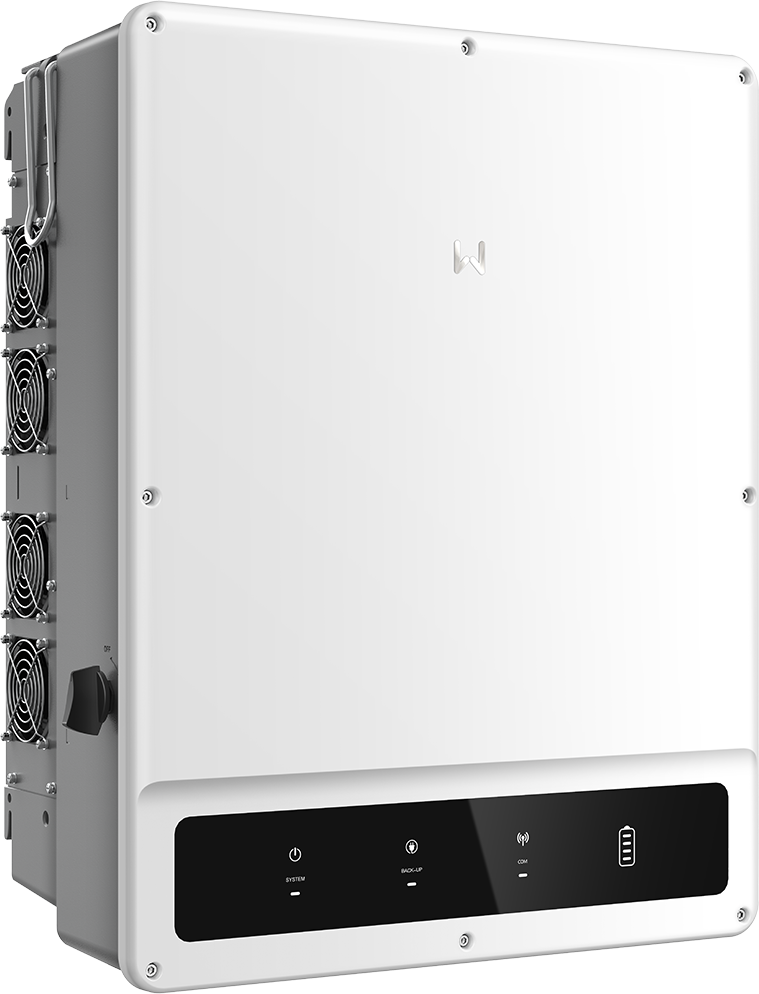
\includegraphics[height=2.6cm]{estaticas/equip-inversor-trifasico.png}\hspace{0.6cm}%
  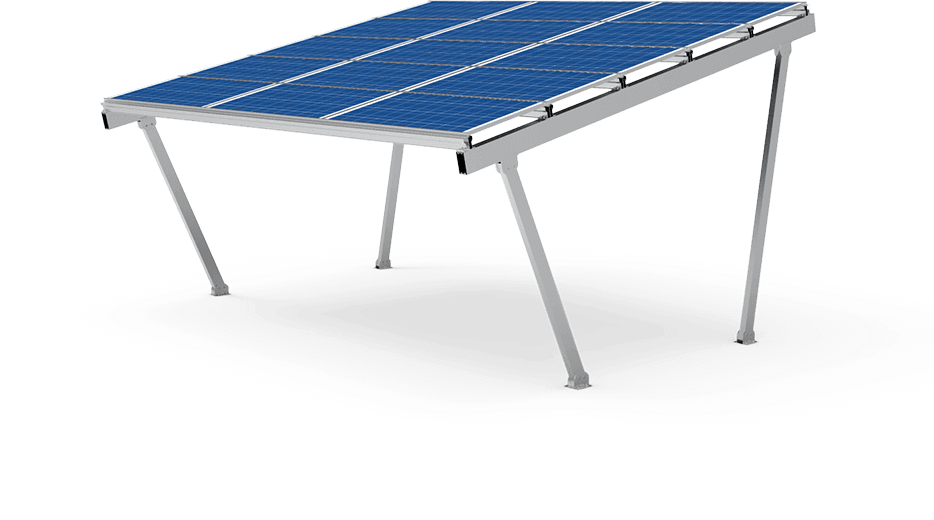
\includegraphics[height=2.6cm]{estaticas/equip-carport.png}%
}

% ---- Números institucionais (slide do monitoramento) -----------------------
\newcommand{\clientesgeridos}{+6.000}
\newcommand{\potenciagerida}{150 MWp}


\begin{document}

% ============================================================================
%  1. Capa
% ============================================================================
\modoescuro
{\usebackgroundtemplate{\fundofoto{estaticas/capa-foto.png}}
\begin{frame}[plain]
  \begin{tikzpicture}[remember picture,overlay]
    \node[anchor=center] at ($(current page.center)+(0,1.35)$)
      {\includegraphics[width=6.2cm]{\logoescura}};
    \node[anchor=south west,text width=13.5cm,align=left,text=brancopace]
      at ($(current page.south west)+(1.1,0.75)$) {%
        {\LARGE\pesosemi\tituloproposta\par}\vspace{0.18cm}
        {\Large\pesomedio\color{amarelopace}\cliente\par}\vspace{0.32cm}
        {\rotulo{Preparado para}\hspace{0.5em}{\small\pesomedio\cliente}\par}\vspace{0.14cm}
        {\rotulo{Data}\hspace{0.5em}{\small\pesoleve\dataproposta}\par}\vspace{0.14cm}
        {\rotulo{Responsável}\hspace{0.5em}{\small\pesoleve\responsavel\ \textperiodcentered\ \responsavelregistro}\par}\vspace{0.1cm}
        {\scriptsize\pesoleve\color{cinzatextoescuro}\responsavelcredenciais\par}
      };
  \end{tikzpicture}
\end{frame}}

% ============================================================================
%  2. Quem somos
% ============================================================================
\begin{frame}{PACE \textbar\ Inteligência Energética}
  \framesubtitle{Integradora das melhores soluções do mercado que gera resultado financeiro com energia}
  \vspace{0.15cm}
  \begin{minipage}[t]{0.55\textwidth}
    \blocotexto{Natureza Consultiva}{Não somos vendedores de equipamentos. Somos consultores focados em gestão estratégica, oferecendo independência técnica para recomendar a melhor solução.}
    \blocotexto{Engenharia de Gestão}{Nossa engenharia vai além da tecnologia. Aplicamos análise de dados e estruturação financeira para transformar energia em uma variável de decisão controlável.}
    \blocotexto{Inteligência Energética}{Focamos na redução de risco e incerteza, estruturando decisões que geram valor real e mensurável para o negócio do cliente.}
  \end{minipage}\hfill
  \begin{minipage}[t]{0.40\textwidth}
    \vspace{0pt}
    \begin{cartao}[top=14pt,bottom=12pt]
      \cartaovalor{\faMedal}{Excelência}{Rigor técnico em análise e recomendação.}\hfill
      \cartaovalor{\faSearch}{Transparência}{Comunicação clara sobre capacidades e limitações.}
      \par\vspace{14pt}
      \cartaovalor{\faHandshake}{Responsabilidade}{Compromisso com a melhor entrega.}\hfill
      \cartaovalor{\faInfinity}{Resultado}{Gerar resultados reais ao cliente.}
    \end{cartao}
  \end{minipage}
\end{frame}

% ============================================================================
%  3. Cases
% ============================================================================
\newcommand{\cartaocase}[5]{%
  % #1 foto principal, #2 foto secundária, #3 ícone, #4 segmento, #5 descrição
  \begin{cartao}[equal height group=cases,width=0.235\textwidth,left=6pt,right=6pt,top=6pt,bottom=8pt]
    \centering
    % As fotos ficam numa caixa de altura fixa: assim o ícone e o título
    % começam na mesma altura em todos os cartões, seja qual for a foto.
    \begin{minipage}[t][3.15cm][t]{\linewidth}\centering
      \ifblank{#2}{%
        \includegraphics[width=\linewidth,height=3.05cm,keepaspectratio]{#1}}{%
        \includegraphics[width=\linewidth,height=1.9cm,keepaspectratio]{#1}\\[3pt]
        \includegraphics[width=\linewidth,height=1.05cm,keepaspectratio]{#2}}
    \end{minipage}\\[6pt]
    \iconecirculo{#3}\\[3pt]
    {\small\pesosemi #4}\\[2pt]
    {\scriptsize\color{cortextosuave}#5}
  \end{cartao}%
}
\begin{frame}{Alguns cases}
  \framesubtitle{Garantindo Inteligência Energética em diversos segmentos}
  \vspace{0.1cm}
  \cartaocase{estaticas/case-logistica-1.jpg}{estaticas/case-logistica-2.png}{\faWarehouse}{Logística}{Galpão Logístico do Exército no RS}\hfill
  \cartaocase{estaticas/case-condominio.png}{}{\faBuilding}{Condomínios}{Economia a custo zero em Memorial -- SP}\hfill
  \cartaocase{estaticas/case-hospital-1.jpg}{estaticas/case-hospital-2.png}{\faHospital}{Hospitais}{Fazenda Solar Exclusiva para 5 Hospitais no RS}\hfill
  \cartaocase{estaticas/case-industria-1.png}{estaticas/case-industria-2.png}{\faIndustry}{Indústrias}{Geração própria e BESS no setor têxtil em SP}
\end{frame}

% ============================================================================
%  4. O sistema proposto
% ============================================================================
\begin{frame}{Geração Fotovoltaica: \cliente}
  \framesubtitle{\subtitulosistema}
  \vspace{0.1cm}
  \begin{minipage}[t]{0.42\textwidth}
    \vspace{0pt}
    \begin{cartao}[left=4pt,right=4pt,top=4pt,bottom=4pt]
      \centering
      \IfFileExists{\fototelhado}{%
        \includegraphics[width=\linewidth,height=4.6cm,keepaspectratio]{\fototelhado}}{%
        % Estudo sem contorno de telhado: a potência veio do consumo, não da
        % área. Dizer isso é melhor que deixar um buraco no slide.
        \begin{minipage}[c][4.6cm]{\linewidth}\centering\color{cortextosuave}
          {\large\faSolarPanel}\\[6pt]
          {\footnotesize Sem contorno de telhado marcado.\\ A potência foi definida pelo consumo.}
        \end{minipage}}
    \end{cartao}
  \end{minipage}\hfill
  \begin{minipage}[t]{0.55\textwidth}
    \vspace{0pt}\centering
    \begin{tabelachave}[3.7cm]{3.2cm}
      \linha{Potência Projeto}{\potenciaprojeto}
      \linha{Potência Módulos}{\potenciamodulo}
      \linha{Quantidade Módulos}{\qtdmodulos}
      \linha{Potência Inversor}{\potenciainversor}
      \linha{Quantidade Inversor}{\qtdinversores}
      \linha{Área Ocupada}{\areaocupada}
      \linha{Produção Anual Esperada}{\producaoanual}
      \linha{BESS}{\bess}
      \linhavisto{Viabilidade Seguro}
      \linhavisto{Viabilidade Gerenciamento}
    \end{tabelachave}
  \end{minipage}
\end{frame}

% ============================================================================
%  5. Monitoramento
% ============================================================================
\newcommand{\cartaomonitor}[3]{%
  % #1 ícone, #2 título, #3 itens (\item ...)
  \begin{cartao}[equal height group=monitor,width=0.31\linewidth,left=7pt,right=7pt]
    \centering\iconecirculo{#1}\\[3pt]
    {\small\pesosemi #2\par}
    \vspace{2pt}{\color{corlinha}\rule{0.8\linewidth}{0.4pt}}\par\vspace{2pt}
    \begin{minipage}{\linewidth}\scriptsize
      \begin{itemize}\setlength{\itemsep}{2pt} #3 \end{itemize}
    \end{minipage}
  \end{cartao}%
}
\begin{frame}{Sistemas geridos com Inteligência Artificial proprietária}
  \framesubtitle{Plataforma CARINA: diagnóstico, gerenciamento e alarme, sem intervenção humana}
  \vspace{0.1cm}
  \begin{minipage}[t]{0.72\textwidth}
    \vspace{0pt}
    \cartaomonitor{\faSearch}{Diagnóstico Inteligente}{\itemvisto Checkup completo pós-entrega; \itemvisto Evita problemas ocultos.}\hfill
    \cartaomonitor{\faClock}{Gerenciamento 24/7}{\itemvisto Exames a cada 5 minutos; \itemvisto IA preditiva.}\hfill
    \cartaomonitor{\faWhatsapp}{Alarmes Automáticos}{\itemvisto Alarmes diretamente no WhatsApp; \itemvisto Ação imediata.}
    \par\vspace{0.35cm}
    {\color{corlinha}\rule{\linewidth}{0.4pt}}\par\vspace{0.2cm}
    \begin{minipage}[c]{0.5\linewidth}
      
\includegraphics[height=0.42cm]{estaticas/carina-logo.png}\hspace{0.25cm}%
      
\includegraphics[height=0.5cm]{estaticas/parceiro-eqi.png}\hspace{0.15cm}%
      
\includegraphics[height=0.5cm]{estaticas/parceiro-solar21.png}\hspace{0.15cm}%
      
\includegraphics[height=0.35cm]{estaticas/parceiro-btg.png}%
    \end{minipage}\hfill
    \begin{minipage}[c]{0.46\linewidth}\raggedleft
      {\large\pesosemi\color{amarelopace}\clientesgeridos}~{\small clientes}\\[2pt]
      {\large\pesosemi\color{amarelopace}\potenciagerida}~{\small sob gestão}
    \end{minipage}
  \end{minipage}\hfill
  \begin{minipage}[t]{0.25\textwidth}
    \vspace{-0.2cm}\centering
    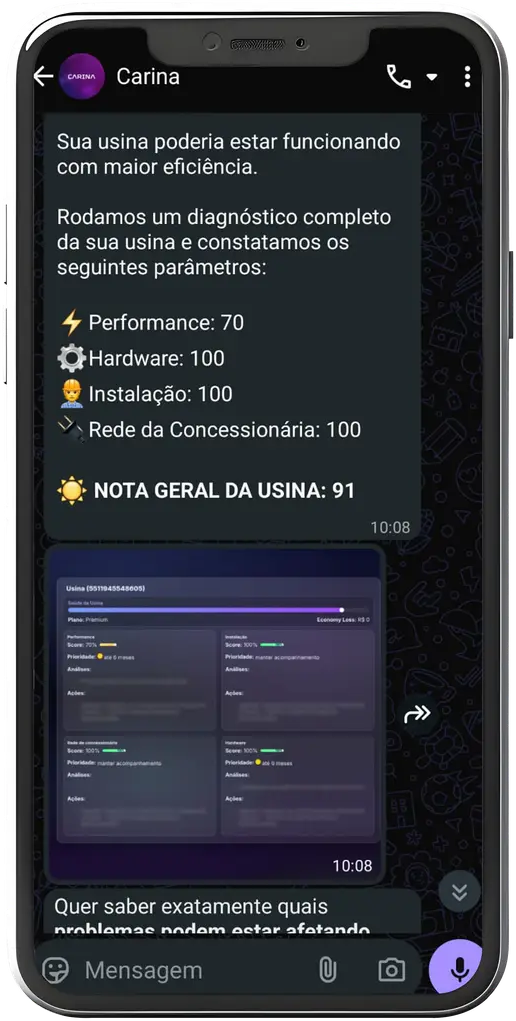
\includegraphics[height=5.6cm]{estaticas/carina-celular.png}
  \end{minipage}
\end{frame}

% ============================================================================
%  5b. O valor do sistema, sem e com bateria — um slide para cada
%
%  São duas compras diferentes: a segunda acrescenta autonomia, não geração.
%  Num slide só, o cliente lê a diferença de preço sem ler o que ela compra.
% ============================================================================
\ifcombateria
\begin{frame}{Sistema sem Bateria -- \cliente}
  \framesubtitle{\notasembateria}
  \vspace{0.05cm}\centering
  \begin{tabelachave}[4.6cm]{4.2cm}
    \linha{Solução}{Gerador solar}
    \linha{Potência do Sistema}{\potenciaprojeto}
    \linha{Geração Anual}{\geracaoanual}
    \linhadestaque{Investimento}{\invsembateria}
    \linha{Economia Anual}{\economiaanualsembateria}
    \linha{Economia Mensal}{\economiamensalsembateria}
    \linha{Mensalidade (\prazofinanciamentocurto)}{\mensalidadesembateria}
    \linha{Payback simples}{\paybacksembateria}
    \linha{Retorno anual (TIR)}{\tirsembateria}
    \linha{Autonomia na falta de energia}{Nenhuma}
  \end{tabelachave}
  \notaderodape{Sem armazenamento, o sistema desliga junto com a rede: é exigência de segurança da norma de conexão, não limitação do equipamento.}
\end{frame}

\begin{frame}{Sistema com Bateria -- \cliente}
  \framesubtitle{\notacombateria}
  \vspace{0.05cm}\centering
  \begin{tabelachave}[4.6cm]{4.2cm}
    \linha{Solução}{Gerador solar + BESS}
    \linha{Potência do Sistema}{\potenciaprojeto}
    \linha{Banco de Baterias}{\bess}
    \linhadestaque{Investimento}{\invcombateria}
    \linha{Diferença para o sem bateria}{\custodabateria}
    \linha{Economia Anual}{\economiaanualcombateria}
    \linha{Mensalidade (\prazofinanciamentocurto)}{\mensalidadecombateria}
    \linha{Payback simples}{\paybackcombateria}
    \linha{Autonomia na falta de energia}{\autonomiacombateria}
  \end{tabelachave}
  \notaderodape{A autonomia é a garantida no pior horário e na pior estação do ano, com a carga do quadro de backup deste estudo.}
\end{frame}
\fi

% ============================================================================
%  6. Compra à vista
% ============================================================================
\begin{frame}{Compra do Sistema -- \cliente}
  \framesubtitle{Aquisição direta -- toda a economia é retorno no seu investimento}
  \vspace{0.05cm}\centering
  \begin{tabelachave}[4.2cm]{4.2cm}
    \linha{Solução}{\solucao}
    \linha{Potência do Sistema}{\potenciaprojeto}
    \linha{Geração Anual}{\geracaoanual}
    \linhadestaque{Investimento Inicial}{\investimento}
    \linha{Economia Anual}{\economiaanual}
    \linha{\rotulopayback}{\payback}
    \linha{Gerenciamento}{\gerenciamentomensal}
    \linha{Seguro}{\seguromensal}
    \linha{\rotulotir}{\tir}
  \end{tabelachave}
  \notaderodape{Para validação da proposta, é necessário que visita técnica comprove que o imóvel tem condições de receber o projeto.}
\end{frame}

% ============================================================================
%  7. Compra financiada
% ============================================================================
\begin{frame}{Compra do Sistema -- \cliente}
  \framesubtitle{Financiamento -- parcelas que reduzem seu investimento}
  \vspace{0.05cm}\centering
  \begin{tabelachave}[4.2cm]{4.2cm}
    \linha{Solução}{Compra Financiada}
    \linhadestaque{Investimento Inicial}{\investimentocurto}
    \linha{Economia Mensal}{\economiamensal}
    \linha{Mensalidade}{\mensalidadefinanciada}
    \linha{Seguro dos Equipamentos}{\segurofinanciado}
    \linha{Gerenciamento}{\gerenciamentofinanciado}
    \linha{Prazo do Contrato}{\prazofinanciamento}
    \linha{Carência}{\carenciafinanciamento}
    \linha{Validade da Proposta}{\validadeproposta}
  \end{tabelachave}
  \notaderodape{Para validação da proposta, é necessário que visita técnica comprove que o imóvel tem condições de receber o projeto.}
\end{frame}

% ============================================================================
%  8. Leasing
% ============================================================================
\begin{frame}{Leasing do Sistema -- \cliente}
  \framesubtitle{As a Service -- investimento ZERO}
  \vspace{0.05cm}\centering
  \begin{tabelachave}[4.2cm]{4.2cm}
    \linha{Solução}{As a Service}
    \linhadestaque{Investimento Inicial}{R\$ 0}
    \linha{Economia Mensal}{\economiamensal}
    \linha{Mensalidade}{\mensalidadeleasing}
    \linhavisto{Seguro dos Equipamentos}
    \linhavisto{Manutenção e Limpeza}
    \linhavisto{Gerenciamento}
    \linha{Prazo do Contrato}{\prazoleasing}
    \linha{Carência}{\carencialeasing}
  \end{tabelachave}
  \notaderodape{Para validação da proposta, é necessário que visita técnica comprove que o imóvel tem condições de receber o projeto.}
\end{frame}

% ============================================================================
%  9. Desembolso mensal
% ============================================================================
\newcommand{\linhadesembolso}[6]{#1 & #2 & #3 & #4 & #5 & #6 \\ \hline}
\begin{frame}{Retorno Financeiro Estimado -- \cliente}
  \framesubtitle{Desembolso mensal, cenário a cenário}
  \vspace{0.4cm}\centering
  \begin{tabeladados}{|\colrotulo{2cm}|*{5}{\colvalor{2.1cm}|}}
    \hline
    \cab{Cenário} & \cab{Investimento inicial} & \cab{Mensalidade} & \cab{Custo mensal} & \cab{Economia mensal} & \cab{Saldo mensal} \\ \hline
    \linhasdesembolso
  \end{tabeladados}
  \notaderodape{\notafluxo}
\end{frame}

% ============================================================================
%  10. Fluxo de caixa acumulado
% ============================================================================
\newcommand{\linhafluxo}[4]{#1 & #2 & #3 & #4 \\ \hline}
\begin{frame}{Retorno Financeiro Estimado -- \cliente}
  \framesubtitle{Fluxo de caixa acumulado}
  \vspace{0.15cm}
  \begin{minipage}[c]{0.46\textwidth}
    \begin{tabeladados}{|\colrotulo{0.6cm}|*{3}{\colvalor{1.7cm}|}}
      \hline
      \cab{Ano} & \cab{À vista} & \cab{Financiado} & \cab{As a Service} \\ \hline
      \linhasfluxo
    \end{tabeladados}
  \end{minipage}\hfill
  \begin{minipage}[c]{0.50\textwidth}
    \raggedleft
    \begin{tikzpicture}
      \begin{axis}[pace,
        width=0.9\linewidth,
        symbolic x coords/.expanded={\fluxoanos},
        xtick=data,xlabel={Ano},
        ylabel={Saldo acumulado (mil R\$)},ylabel near ticks,
        ylabel style={font=\tiny,color=cortextosuave},
        enlarge y limits=0.08,
      ]
        \addplot coordinates {\fluxoavista};\addlegendentry{À vista}
        \addplot coordinates {\fluxofinanciado};\addlegendentry{Financiado}
        \addplot coordinates {\fluxoservico};\addlegendentry{As a Service}
        \addplot[dashed,cortextosuave,mark=none,forget plot] coordinates {\fluxozero};
      \end{axis}
    \end{tikzpicture}
  \end{minipage}
  \notaderodape{\notafluxo}
\end{frame}

% ============================================================================
%  11. Fecho
% ============================================================================
{\usebackgroundtemplate{\fundofoto{estaticas/capa-foto.png}}
\begin{frame}[plain]
  \begin{tikzpicture}[remember picture,overlay]
    \node[anchor=center,text=brancopace,align=center,font=\Large\pesoleve,text width=13cm]
      at ($(current page.center)+(0,1.6)$)
      {Energia deixou de ser apenas conta.\\[3pt]{\pesosemi Tornou-se estratégia.}};
    \node[anchor=center] at ($(current page.center)+(0,-0.9)$)
      {\includegraphics[width=5.6cm]{\logoescura}};
  \end{tikzpicture}
\end{frame}}

% ============================================================================
%  12. Divisor
% ============================================================================
\slidedivisor{Informações adicionais}{Como escolhemos o que instalamos}

% ============================================================================
%  13. Alta qualidade
% ============================================================================
\modoclaro
\newcommand{\cartaofator}[2]{%
  \begin{minipage}[t]{0.31\textwidth}
    \centering{\small\pesosemi #1\par}\vspace{4pt}
    \begin{cartao}[equal height group=fatores,top=10pt,bottom=10pt]
      \begin{minipage}{\linewidth}\footnotesize
        \begin{itemize}\setlength{\itemsep}{5pt} #2 \end{itemize}
      \end{minipage}
    \end{cartao}
  \end{minipage}%
}
\begin{frame}{Alta qualidade}
  \framesubtitle{Trabalhamos com equipamentos de \colorbox{amarelopace}{\textcolor{pretopace}{\pesosemi primeira linha}}}
  \vspace{0.2cm}
  {\small\pesosemi 3 principais fatores avaliados:\par}
  \vspace{0.3cm}
  \cartaofator{Avaliação PACE}{\item Desmontamos a maioria dos equipamentos do Brasil; \item Usinas próprias há mais de 8 anos; \item Gerenciamos mais de 140 MWp pelo Brasil.}\hfill
  \cartaofator{Certificados}{\item Marcas e modelos que passaram pelos mais rigorosos testes internacionais de qualidade; \item Tier 1 não avalia qualidade, e sim bancabilidade.}\hfill
  \cartaofator{Pós-venda no Brasil}{\item Marcas com escritório no Brasil; \item Proximidade com fabricante na China; \item Pós-venda rápido e assertivo.}
\end{frame}

% ============================================================================
%  14. Certificações
% ============================================================================
\newcommand{\certificacao}[3]{%
  % #1 logo, #2 altura da logo, #3 texto
  \begin{cartao}[left=6pt,right=8pt,top=3pt,bottom=3pt,boxsep=0pt]
    \begin{minipage}[c]{1.3cm}\centering\includegraphics[height=#2,width=1.2cm,keepaspectratio]{#1}\end{minipage}\hfill
    \begin{minipage}[c]{0.88\linewidth}\scriptsize #3\end{minipage}
  \end{cartao}\par\vspace{3pt}
}
\begin{frame}{Certificações}
  \framesubtitle{Avaliamos marcas e modelos anualmente com base nos certificados}
  \vspace{0.05cm}
  \certificacao{estaticas/cert-retc.png}{0.42cm}{\textbf{RETC.} Laboratório americano independente de testes e certificação para módulos, inversores e baterias. Seus laudos comprovam qualidade e bankability do produto.}
  \certificacao{estaticas/cert-pvel.png}{0.42cm}{\textbf{PVEL.} Laboratório independente que testa durabilidade e desempenho real de módulos fotovoltaicos fora das condições de laboratório padrão.}
  \certificacao{estaticas/cert-ce.png}{0.5cm}{\textbf{CE.} Obrigatório para venda na Europa. Atesta que módulos, inversores e baterias cumprem requisitos de segurança, saúde e proteção ambiental da UE.}
  \certificacao{estaticas/cert-ul.png}{0.5cm}{\textbf{UL.} Certificação de segurança americana. Exigida para o mercado dos EUA em módulos (UL 61730), inversores (UL 1741) e baterias (UL 9540).}
  \certificacao{estaticas/cert-tuv.png}{0.55cm}{\textbf{TÜV.} Organismo alemão de inspeção e testes. Certifica segurança elétrica e mecânica de módulos e inversores, reconhecido mundialmente como padrão de qualidade.}
  \certificacao{estaticas/cert-tier1.png}{0.5cm}{\textbf{Tier 1.} Classificação financeira da Bloomberg do fabricante de módulos, não do produto. Indica solidez da empresa e capacidade de honrar garantias de 25+ anos.}
  \certificacao{estaticas/cert-inmetro.png}{0.5cm}{\textbf{INMETRO.} Instituto Nacional de Metrologia do Brasil. Certificação obrigatória no mercado brasileiro para módulos fotovoltaicos e inversores.}
\end{frame}

% ============================================================================
%  15. Equipamentos e garantias
% ============================================================================
\begin{frame}{Equipamentos e garantias}
  \framesubtitle{O que cobre cada família de equipamento}
  \vspace{0.15cm}\centering
  \begin{tabeladados}{|\colrotulo{3.4cm}|*{4}{\colvalor{2.2cm}|}}
    \hline
    \cab{Equipamento} & \cab{Inversor} & \cab{BESS} & \cab{Módulo} & \cab{Carregador} \\ \hline
    Garantia de Fabricação & 10 anos & 5 anos & 10 anos & 5 anos \\ \hline
    Garantia de Performance & 10 anos & 16 mil ciclos & 20 anos & -- \\ \hline
  \end{tabeladados}
  \par\vspace{0.4cm}
  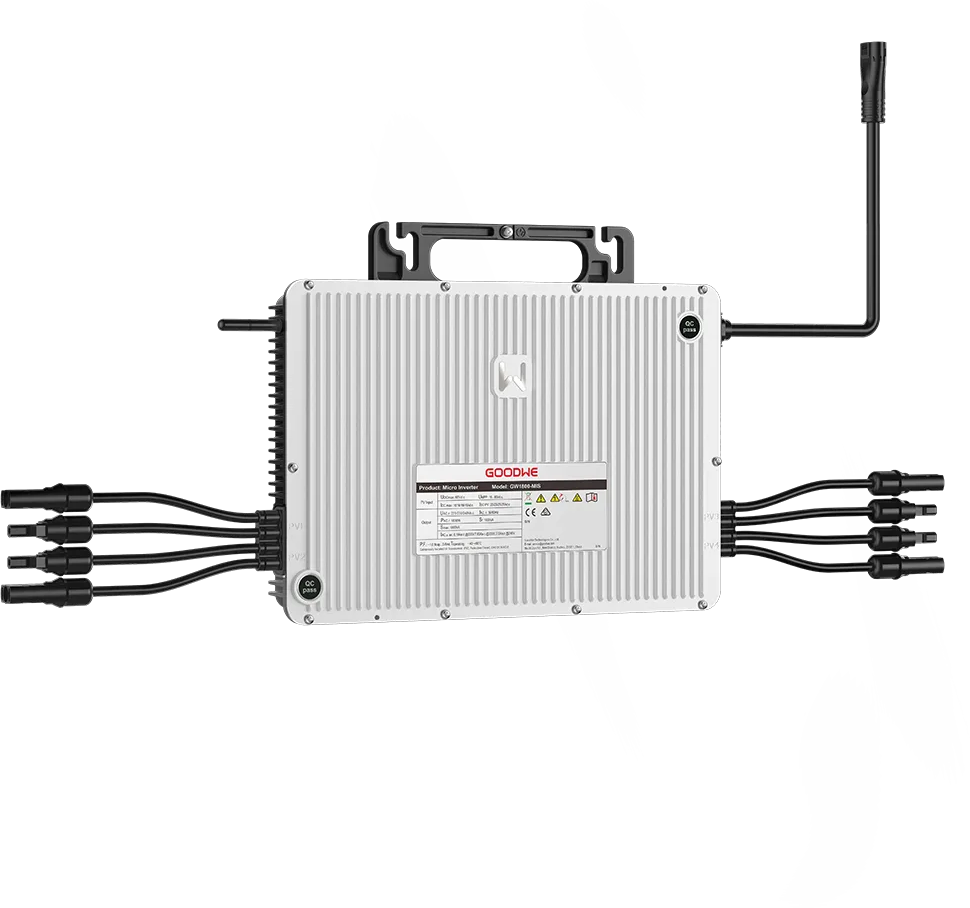
\includegraphics[height=1.7cm]{estaticas/equip-microinversor.png}\hspace{0.25cm}%
  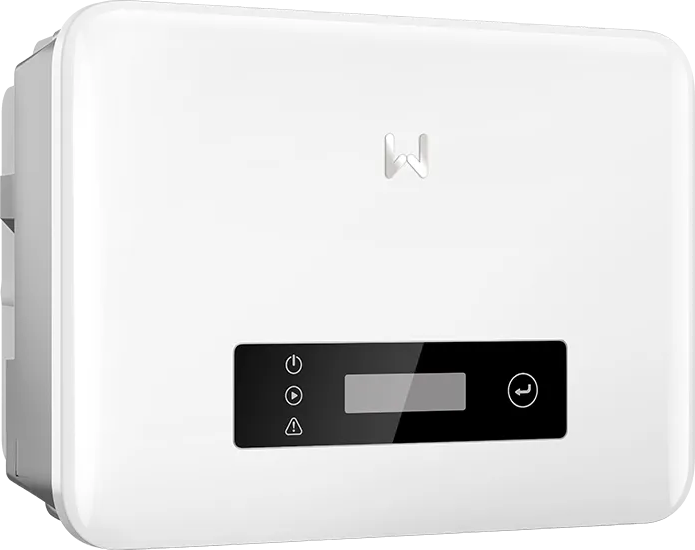
\includegraphics[height=1.7cm]{estaticas/equip-inversor-string.png}\hspace{0.25cm}%
  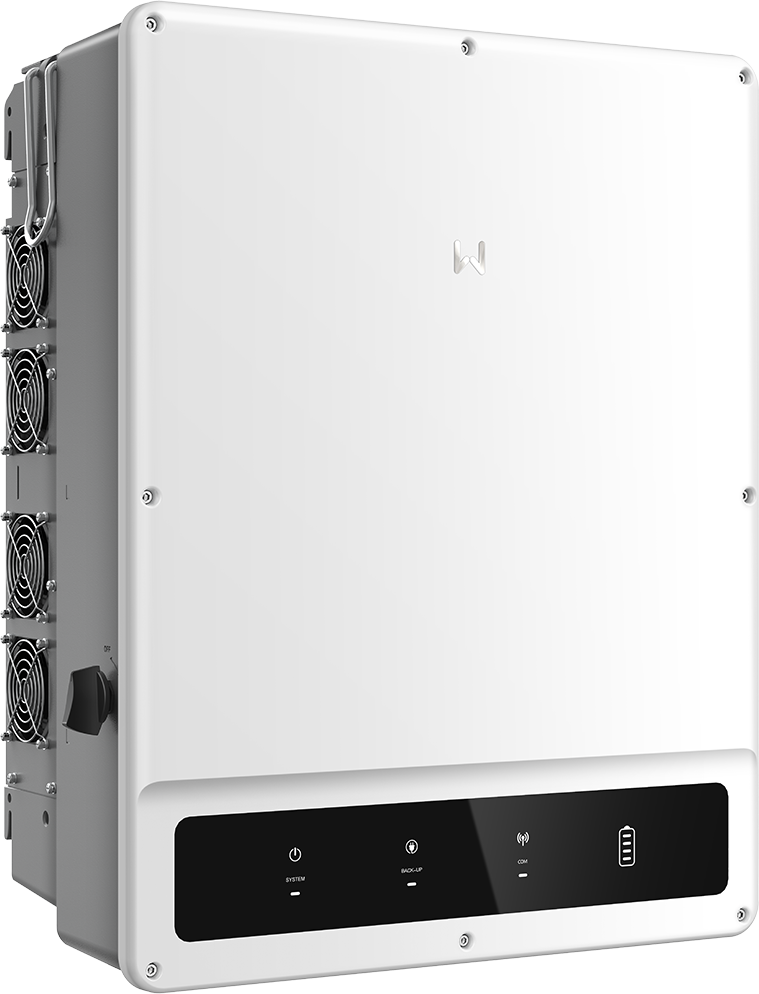
\includegraphics[height=1.7cm]{estaticas/equip-inversor-trifasico.png}\hspace{0.5cm}%
  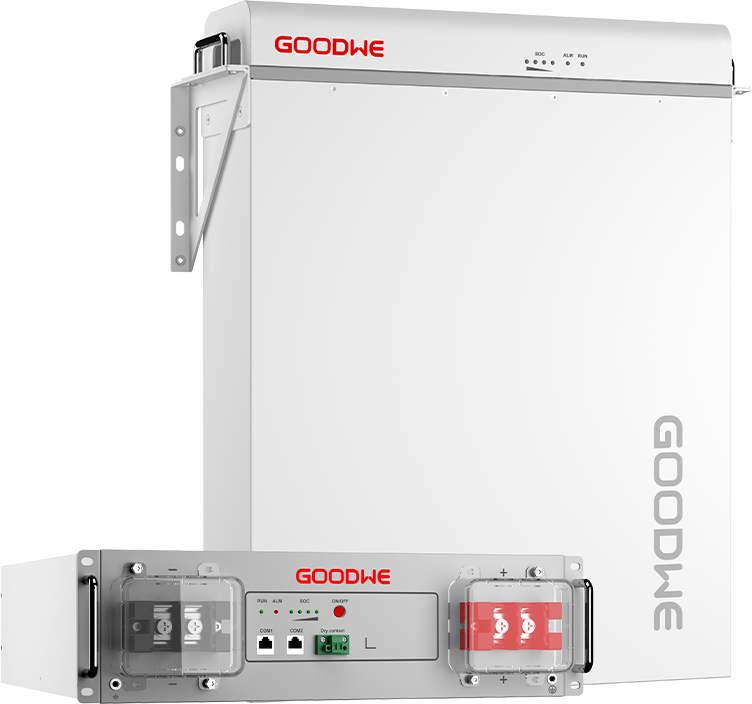
\includegraphics[height=1.7cm]{estaticas/equip-bess-parede.png}\hspace{0.25cm}%
  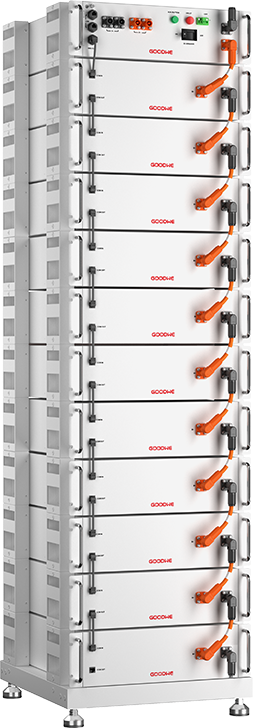
\includegraphics[height=1.7cm]{estaticas/equip-bess-rack.png}\hspace{0.25cm}%
  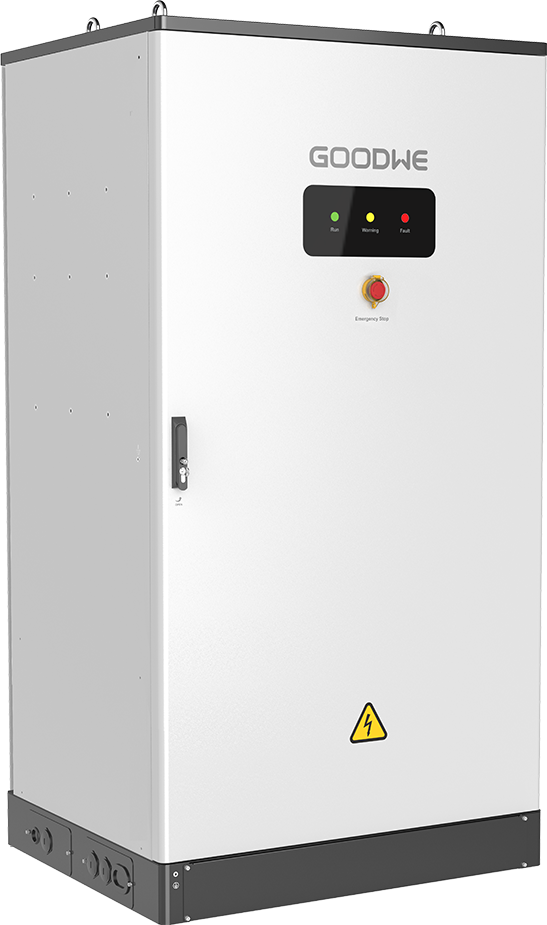
\includegraphics[height=1.7cm]{estaticas/equip-bess-cabine.png}\hspace{0.5cm}%
  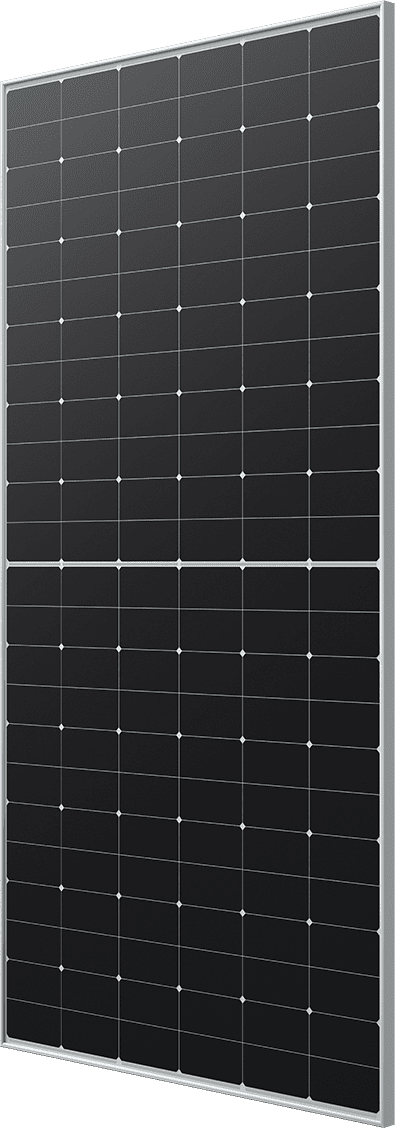
\includegraphics[height=1.7cm]{estaticas/equip-modulo.png}\hspace{0.5cm}%
  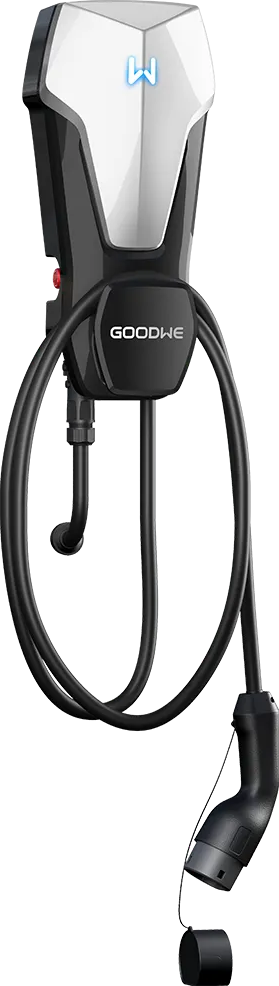
\includegraphics[height=1.7cm]{estaticas/equip-carregador.png}
  \par\vspace{0.1cm}
  {\tiny\color{cortextosuave}Inversores \textperiodcentered\ Armazenamento (BESS) \textperiodcentered\ Módulos \textperiodcentered\ Carregador veicular\par}
\end{frame}

% ============================================================================
%  16. Bancos parceiros
% ============================================================================
\newcommand{\banco}[2]{\includegraphics[height=#2,width=1.7cm,keepaspectratio]{#1}}
\begin{frame}{Bancos parceiros}
  \framesubtitle{Linhas de financiamento já negociadas para os nossos projetos}
  \vspace{0.3cm}\centering
  \begin{tabeladados}{|\collogo{2.2cm}|*{3}{\colvalor{3.2cm}|}}
    \hline
    \cab{Banco} & \cab{Prazo} & \cab{Carência} & \cab{Modelo} \\ \hline
    \banco{estaticas/banco-cashme.png}{0.32cm} & Até 90 meses & Até 3 meses & Financiamento p/ condomínios \\ \hline
    \banco{estaticas/banco-bv.png}{0.55cm} & Até 90 meses & Até 4 meses & Financiamento PF e PJ \\ \hline
    \banco{estaticas/banco-solagora.png}{0.3cm} & Até 90 meses & Até 4 meses & Financiamento PF e PJ \\ \hline
    \banco{estaticas/banco-santander.png}{0.3cm} & Até 90 meses & Até 3 meses & Financiamento PF e PJ \\ \hline
    \banco{estaticas/banco-solfacil.png}{0.38cm} & Até 120 meses & Até 4 meses & Financiamento PF e PJ \\ \hline
  \end{tabeladados}
  \par\vspace{0.4cm}
  {\footnotesize\pesosemi Taxas aprovadas dependem da qualidade de crédito do cliente.\par}
\end{frame}

% ============================================================================
%  17. Divisor
% ============================================================================
\slidedivisor{Anexo}{Lista de equipamentos e próximos passos}

% ============================================================================
%  18. Lista de equipamentos
% ============================================================================
\modoclaro
\newcommand{\linhaequipamento}[5]{#1 & #2 & #3 & #4 & #5 \\ \hline}
\begin{frame}{Lista de equipamentos}
  \framesubtitle{O que compõe o sistema proposto para \cliente}
  \vspace{0.3cm}\centering
  \begin{tabeladados}{|\colrotulo{2.2cm}|*{4}{\colvalor{2.3cm}|}}
    \hline
    \cab{Equipamento} & \cab{Marca} & \cab{Quantidade} & \cab{Potência} & \cab{Garantia} \\ \hline
    \linhasequipamentos
  \end{tabeladados}
  \par\vspace{0.5cm}
  \fotosequipamentos
\end{frame}

% ============================================================================
%  19. Próximos passos
% ============================================================================
\modoescuro
\begin{frame}{Próximos passos}
  \framesubtitle{Da aprovação à energia na tomada}
  \begin{tikzpicture}[remember picture,overlay]
    \foreach \x/\icone/\rotulo in {
        1.9/\faUsers/Aprovações,
        4.6/\faFileSignature/Assinatura do contrato,
        7.3/\faHardHat/Instalação,
        10.0/\faStamp/Homologação na concessionária,
        12.7/\faBolt/Ativação do sistema} {
      \node (p) at ($(current page.south west)+(\x+0.65,4.3)$) {\iconepasso{\icone}};
      \node[below=0.25cm of p,text width=2.4cm,align=center,font=\footnotesize\pesosemi,text=brancopace] {\rotulo};
    }
    \foreach \x in {3.25,5.95,8.65,11.35} {
      \node[text=amarelopace,font=\Large] at ($(current page.south west)+(\x+0.65,4.3)$) {\faAngleDoubleRight};
    }
  \end{tikzpicture}
\end{frame}

\end{document}
